\documentclass[boldfont,linespread=1.35]{ctexart}
\usepackage{geometry}%用于调整页面大小
\geometry{a4paper,scale=0.75}
\usepackage{amsmath}
\usepackage{colortbl,booktabs}%表格
\usepackage{graphicx}%用于插入图片,下同
\usepackage{float}
\usepackage{xcolor}
\setCJKmainfont{楷体}

\title{\textbf{
		\zihao{1}鉴别伪造图片\\
		\zihao{2}人工智能思维与伦理课程大作业
	}}
\author{\textbf{王凯灵521030910356}}
\date{\textbf{2021.10.7}}
\pagestyle{plain}

\begin{document}

	\maketitle
	\zihao{5}
\section{理解含义}
\subsection{精确率和召回率}
精确率,顾名思义,很好理解,即模型在真假判断中答对的概率。召回率,我猜想,可能是测试集中正类标签项答对的概率。如果是这样,在样本足够大时,这两个值理应相差不大。

于是标记了所有的样本,在训练集占比0.8的情况下试训练了第一次模型,结果图1:
\begin{figure}[h]
	\centering
	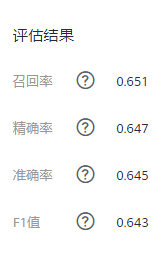
\includegraphics[width=3.5cm]{screenshot001}
	\color{gray}\caption{ 第一次训练}
\end{figure}

可见,精确率与召回率确实相差无几。图2数据也符合预期。

\begin{figure}[h]
	\centering
	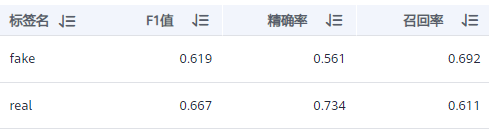
\includegraphics[width=10 cm]{screenshot002}
	\color{gray}\caption{也是第一次训练}
\end{figure}

于是我查看公式验证自己的猜想,发现精确率理解无差,但发现召回率并不是我想的那样。事实上,召回率代表系统在输入的数据集中正确判断并找出的正类样本占所有输入正类样本的比。以此次输入为例,标签real的召回率就是测试时,模型标记对的real数量除以测试集的总real量。确实,这样定义更符合“召回”。

\subsection{$F_{1}$值}
根据公式,$F_{1}$值即精确率与召回率的调和平均。就公式来看,这显然是反映模型综合能力的数据。关于这样计算的含义,我给出以下思路:

考虑label1精确率很高,但召回率不高。可知label2召回率高而精确率不高。模型存在“偏科现象”此时$F_{1}$值都较接近精确率和召回率中较低的一个。这样既考虑了模型对不同label分辨能力差异导致的综合能力偏低,又考虑了模型对某一label存在的特长。

根据这种想法,实际应用过程中往往对精确率和召回率有一定要求,其中某一个较为重要,但又不能忽视另一个。所以根据不同的要求和$F_{1}$这个名字,我断定还有$F_{n}$根据不同侧重点而变化。

查证,定义有
$F_{\beta}=\left(1+\beta^{2}\right) \cdot \frac{\textit { precision } \cdot \textit { recall }}{\left(\beta^{2} \cdot \textit { precision }\right)+\textit { recall }}$

然而,就当前判断图片真假的模型,我并不觉得$F_{\beta}$有多大用。但是华为云平台并没有自主更改$\beta$的选择,笔者以为不太合理。\\

此后,又发现了精确率和准确率的区别。具体来说,精确率是指模型认为是某一label的图片有多少确实是这一label,而准确率是指所有预测里正确所占的比例。笔者语文不好,可以说乱七八糟的知识增加了\ldots

\section{训练尝试}
\subsection{改变训练比}
由之前的数据,0.8的训练比准确率低于0.7,显然这不太让人满意。

于是改变训练比,从0.1至0.9,所得准确率值依次为:

\begin{table} [h]
	\centering
	\caption{训练比与准确率}
	\begin{tabular}
		{cccccccccc}
		\toprule[1pt]
		\rowcolor[gray]{0.9} 训练比 &0.1 &0.2 &0.3 &0.4 &0.5 &0.6 &0.7 &0.8 &0.9\\
		\midrule
		准确率   &0.627 &0.613 &0.589 &0.643 &0.591 &0.674 &0.607 &0.645 &0.695\\
		\bottomrule[1pt]
	\end{tabular}
\end{table}

该说姜还是老的辣吧,0.9的训练比准确率最高。但是又考虑到训练集或者测试集越来越小,偶然性很可能增加。于是我部署了训练比为0.1、0.9和0.5的三个模型,准备进行进一步测试。

测试发现,对于CASIA中的样本,0.1模型错误率明显高于0.5和0.9。说实话,0.5模型的正确相当不错,故暂且认为不平衡的训练集和测试集会导致准确率的误差。另一方面,发现在所有的测试中,笔者在此定义“把握”(confidence)$:=2\left|0.5-score(real)\right|$,0.1和0.5模型对于图片都有非常高的把握,这个数据基本稳定在0.5以上(虽然结果并不一定是对的),而0.9模型的把握往往极低,只有0.1左右。我思索良久,我悟了。AI正如人类一样,在年少轻狂时候往往说一不二,行事果断。而到了真正见多识广的年纪,却瞻前顾后,优柔寡断。这对我学习人工智能思维与伦理又有了新的(奇怪的)启发。

我的头像是由于我因事缺席宣传部团建拍照,深感惋惜,于是自己缝合了多张图像做出的图片,在宣传部内部可以假乱真。

于是,我用我自己来测试这三个模型:
\begin{figure}[h]
	\centering
	{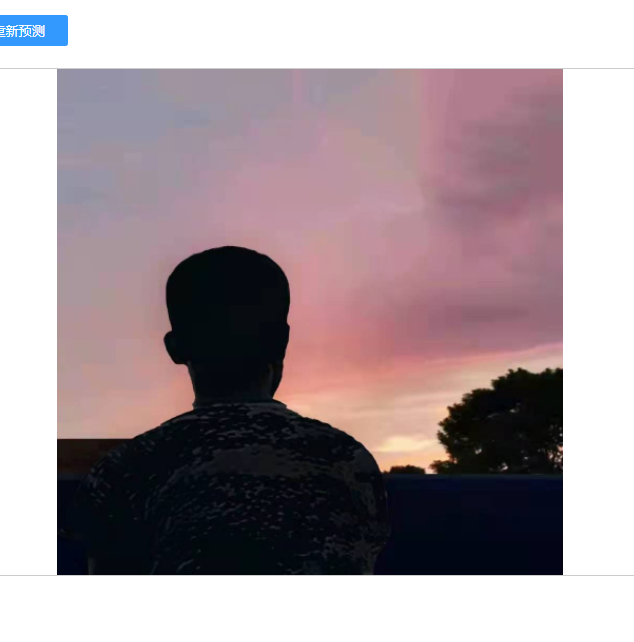
\includegraphics[width=5cm]{11}}
	{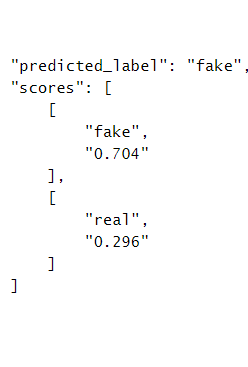
\includegraphics[width=3cm]{22}}
	{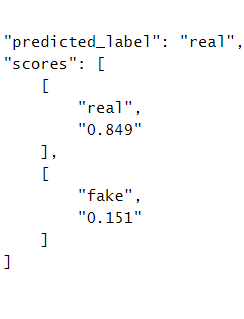
\includegraphics[width=3cm]{33}}
	{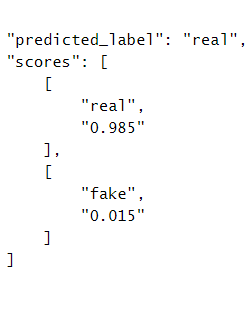
\includegraphics[width=3cm]{44}}
	\color{gray}\caption{头像测试结果,从左到右0.9、0.5、0.1}
\end{figure}

结果依旧服从后两个模型把握较高的规律,以及我十分感激这两位对我PS技术的信赖和认可。

综上发现,当我改变训练比的时候,模型总体性能并没有太大改变,至少没有明显的线性关系。而且整体水平并不高。特定图片,不同模型给出判断有明显差异。这已经排除了这张图片属于训练集、训练集各类图片数量不均的情况。

\subsection{改变真伪比}
为控制变量,训练比统一为默认的0.8。总样本为600,本别进行了真伪1:1,1:2,2:1的训练。结果如下:
\begin{table} [h]
	\centering
	\caption{真伪比与准确率}
	\begin{tabular}
		{cccc}
		\toprule[1pt]
		\rowcolor[gray]{0.9} 真伪比 &1:1 &1:2 &2:1\\
		\midrule
		准确率   &0.625 &0.750 &0.703\\
		\bottomrule[1pt]
	\end{tabular}
\end{table}

如果单从数据上来看,不平衡的真伪比提高了模型的准确率。于是再次进行随机测试。大量尝试后,发现真伪比为1:2和2:1的两个模型相较于1:1的模型而言,更容易出现高把握的错误。其中,真样本较多的模型倾向于认为假的是真的,假样本较多的反之。为了进一步确认这一规律,我特地挑出了一些显然是真的图片和离谱的假图:
\begin{figure}[h]
	\centering
	{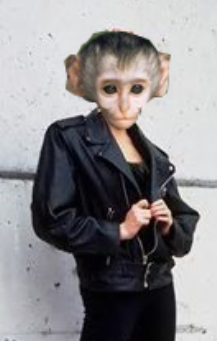
\includegraphics[width=4cm]{111}}
	{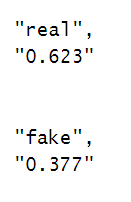
\includegraphics[width=3cm]{112}}
	{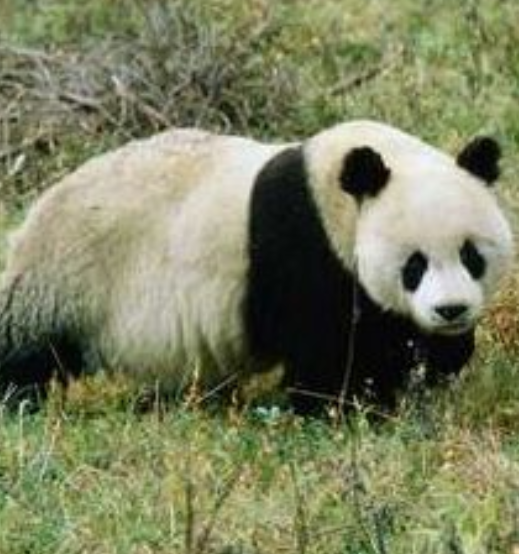
\includegraphics[width=4cm]{113}}
	{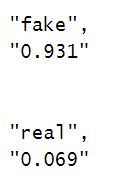
\includegraphics[width=3cm]{114}}
	\hspace{0in}
	\color{gray}\caption{测试结果,左为2:1模型结果,右为1:2模型结果}
\end{figure}

当然头像也要再来一遍:
\begin{figure}[h]
	\centering
	{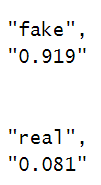
\includegraphics[width=2cm]{1111}}
	{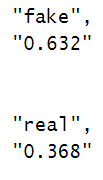
\includegraphics[width=2cm]{1112}}
	{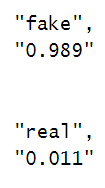
\includegraphics[width=2cm]{1113}}
	\color{gray}\caption{第二次头像测试,从左至右:1:1,2:1,1:2}
\end{figure}

看来他们面对我意外的一致\ldots

这里,我又产生了一些想法。当人的视野有偏差,或是被锁在信息茧房中,或是被潮流误导,或是被局限在幸福的生活中,而忘了艰苦的岁月(有感而发),人也难免做出不正确的判断。果然,AI模型也是如此。

最终,我根据其余大量的测试,最后选择了一个总样本800,训练比0.8,真伪比1:1的模型,进行进一步试验。

\section{观察与分析}
我选取的最终模型四项参考数据均为0.708,我以这个模型为基准,辅以其他部署完的几十个模型抽取检验。这个模型准确率不是最高的,但经过试验,发现所有离谱的错误预测结果都是正确的。这就避免了我胡扯。于是我选取了以下几个典型错误:
\subsection{有模糊前景}
说实话我也看了一会才明白过来。我认为此处模糊的前景和模糊的奇怪的东西混在了一起,迷惑了AI。
\begin{figure}[h]
	\centering
	{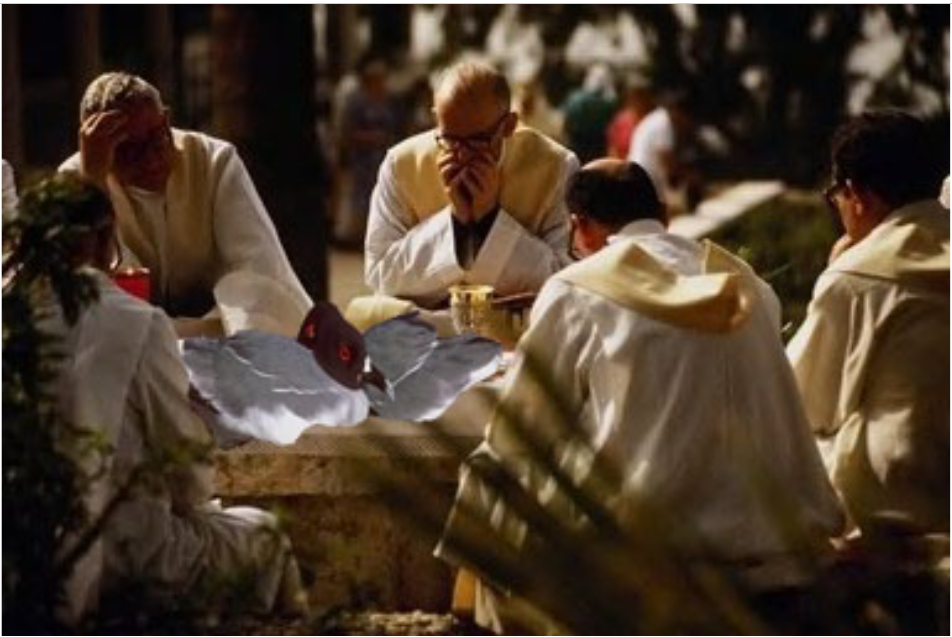
\includegraphics[width=8cm]{1}}
	{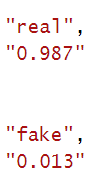
\includegraphics[width=2cm]{2}}
	\color{gray}\caption{模糊前景}
\end{figure}
\subsection{颜色类似,边缘平滑}
这张图有着相当合理的结构,边缘由于颜色相似而并不明显。抠图抠的也干净。
\begin{figure}[h]
	\centering
	{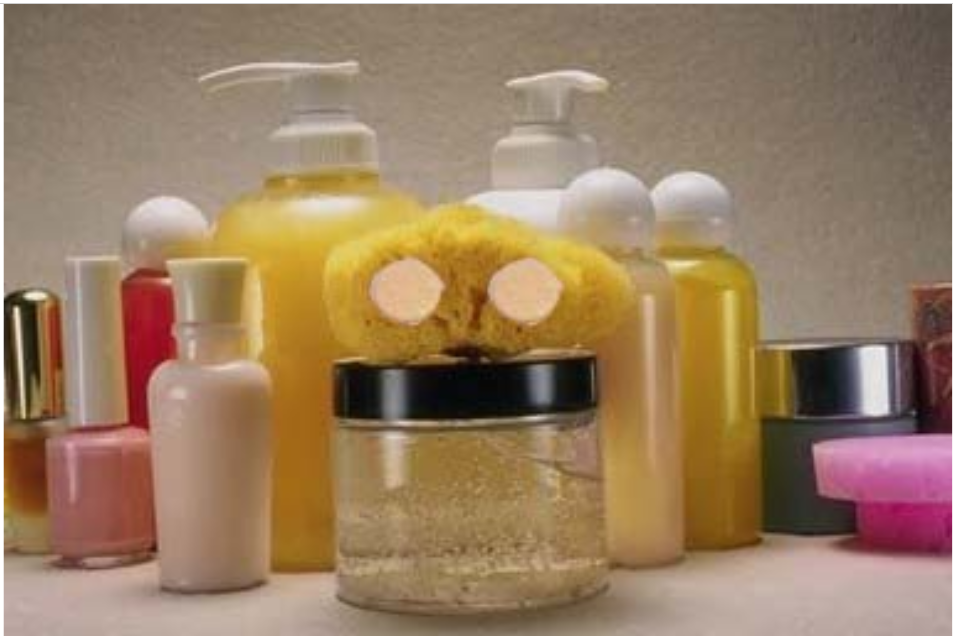
\includegraphics[width=8cm]{3}}
	{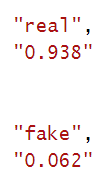
\includegraphics[width=2cm]{4}}
	\color{gray}\caption{色近边顺}
\end{figure}
\subsection{过于模糊或羽化效果}
和上面一例类似但不同。考虑到可以通过算法计算边缘,羽化效果的滤波器能产生与之对抗的效果,是计算机认为物体和周围是一体的。太过模糊的图片本质上和羽化是类似的。
\begin{figure}[h]
	\centering
	{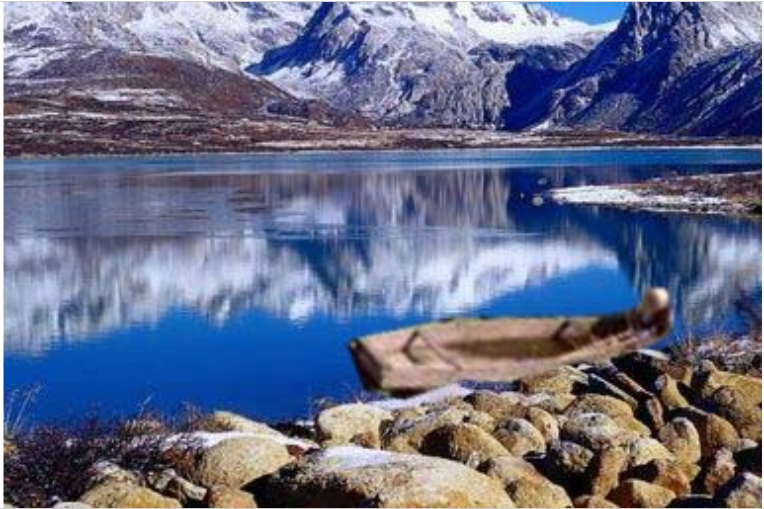
\includegraphics[width=8cm]{5}}
	{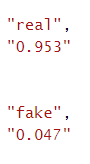
\includegraphics[width=2cm]{6}}
	\color{gray}\caption{太糊了}
\end{figure}
\subsection{制图者高超的本领}
不必我多说了吧。(其实很可能是因为太糊了)
\begin{figure}[h]
	\centering
	{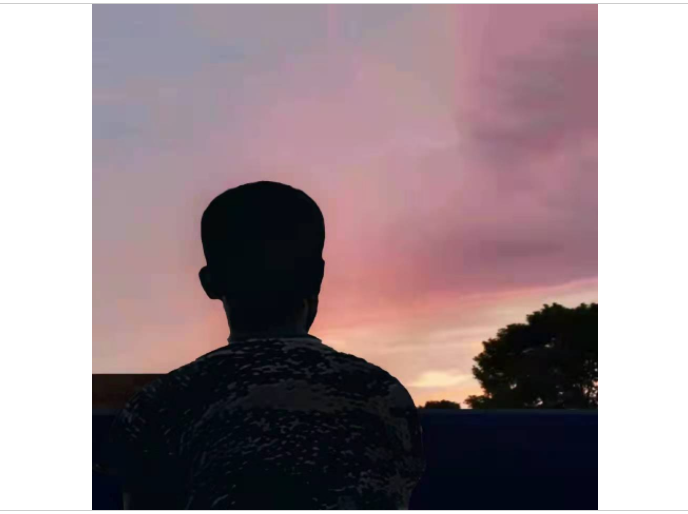
\includegraphics[width=8cm]{7}}
	{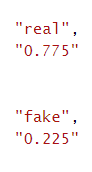
\includegraphics[width=2cm]{8}}
	\color{gray}\caption{诶嘿}
\end{figure}

下面找出几个真判假的例子:
\subsection{界限分明,颜色突出}
和羽化效果相对,这种图片产生了分明的界限,所以很可能判假。
\begin{figure}[h]
	\centering
	{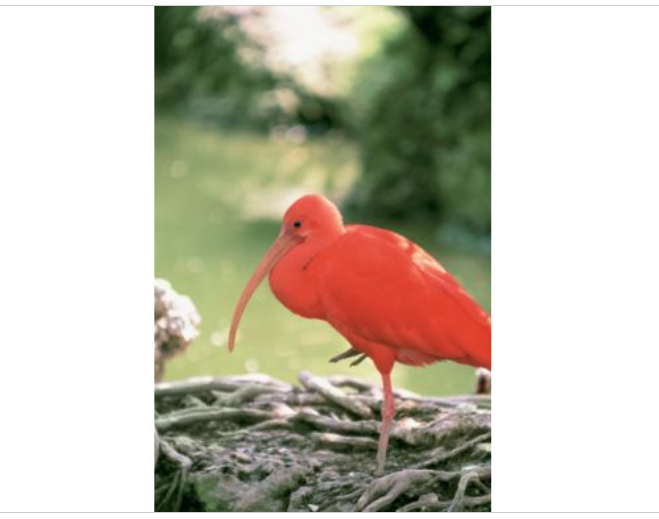
\includegraphics[width=6cm]{9}}
	{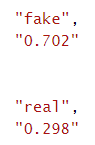
\includegraphics[width=2cm]{10}}
	\color{gray}\caption{界限分明}
\end{figure}

\begin{figure}[h]
	\centering
	{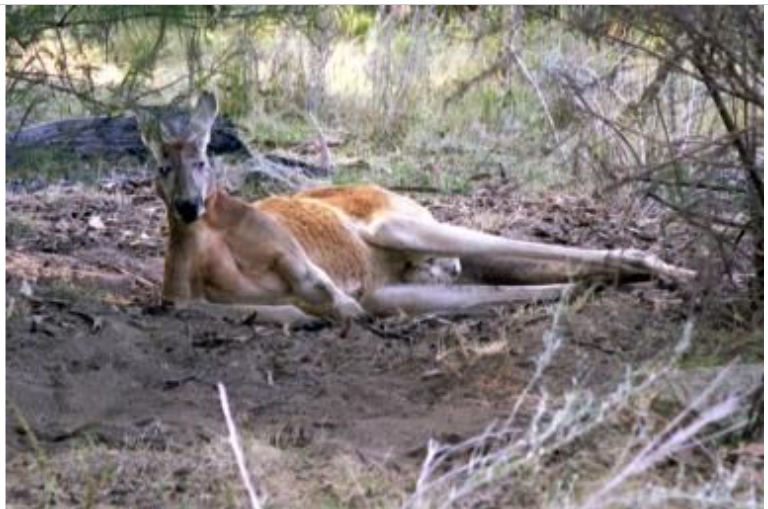
\includegraphics[width=6cm]{12}}
	{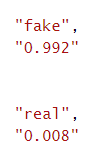
\includegraphics[width=2cm]{13}}
	\color{gray}\caption{同样界限分明}
\end{figure}

\newpage
\subsection{这是为啥}
我快绷不住了
\begin{figure}[h]
	\centering
	{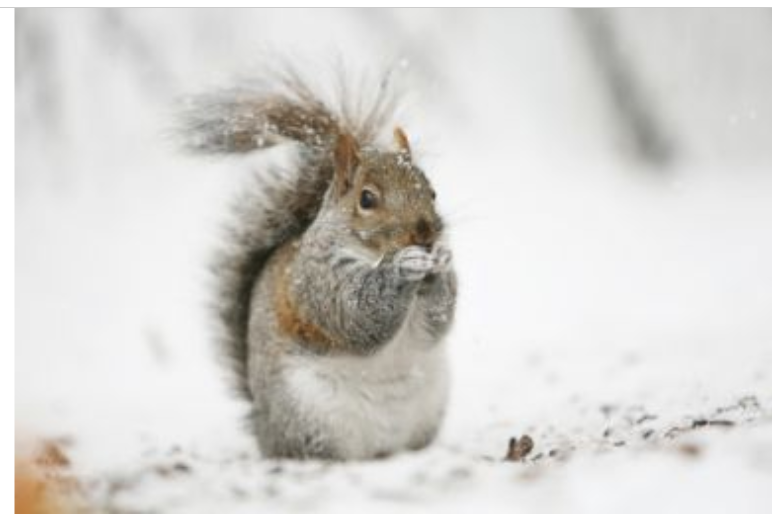
\includegraphics[width=6cm]{14}}
	{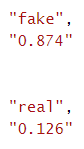
\includegraphics[width=2cm]{15}}
	\color{gray}\caption{???}
\end{figure}

这么多图看下来,我还是认为图片清晰度要背锅。杂乱的像素点降低了模型的准确率。而且,就数据来看,real图片清晰度相对于fake图片更低,所以清晰度更接近fake图片的,更有可能北屋盘,比如这只松鼠。

为了进一步测试模型性能和寻找其他因子,我用朋友圈的图片(已取得本人同意)做了一组清晰度更符合实际生活场景的真假图片:

\section{控制变量测试}
以下是原图(图13):
\begin{figure}[h]
	\centering
	\includegraphics[width=0.6\linewidth]{../测试图/测试原图}
	\color{gray}\caption{测试原图}
\end{figure}

\subsection{整体处理}
在此基础上,我又制作了按照训练集清晰度模糊化的原图(图14)和使用Topaz Sharpen AI自动加工(去除噪点,锐化等)的原图(图15)
\begin{figure}[h]
	\centering
	\begin{minipage}[t]{0.45\linewidth}
		\centering
		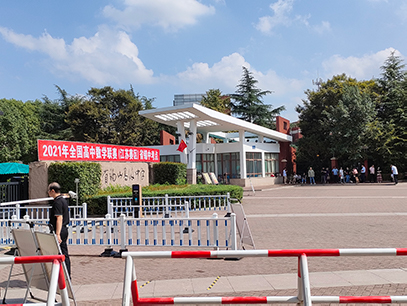
\includegraphics[width=6cm]{../测试图/测试模糊}
		\color{gray}\caption{测试模糊}
	\end{minipage}
	\begin{minipage}[t]{0.45\linewidth} %图片占用一行宽度的45%
		\centering
		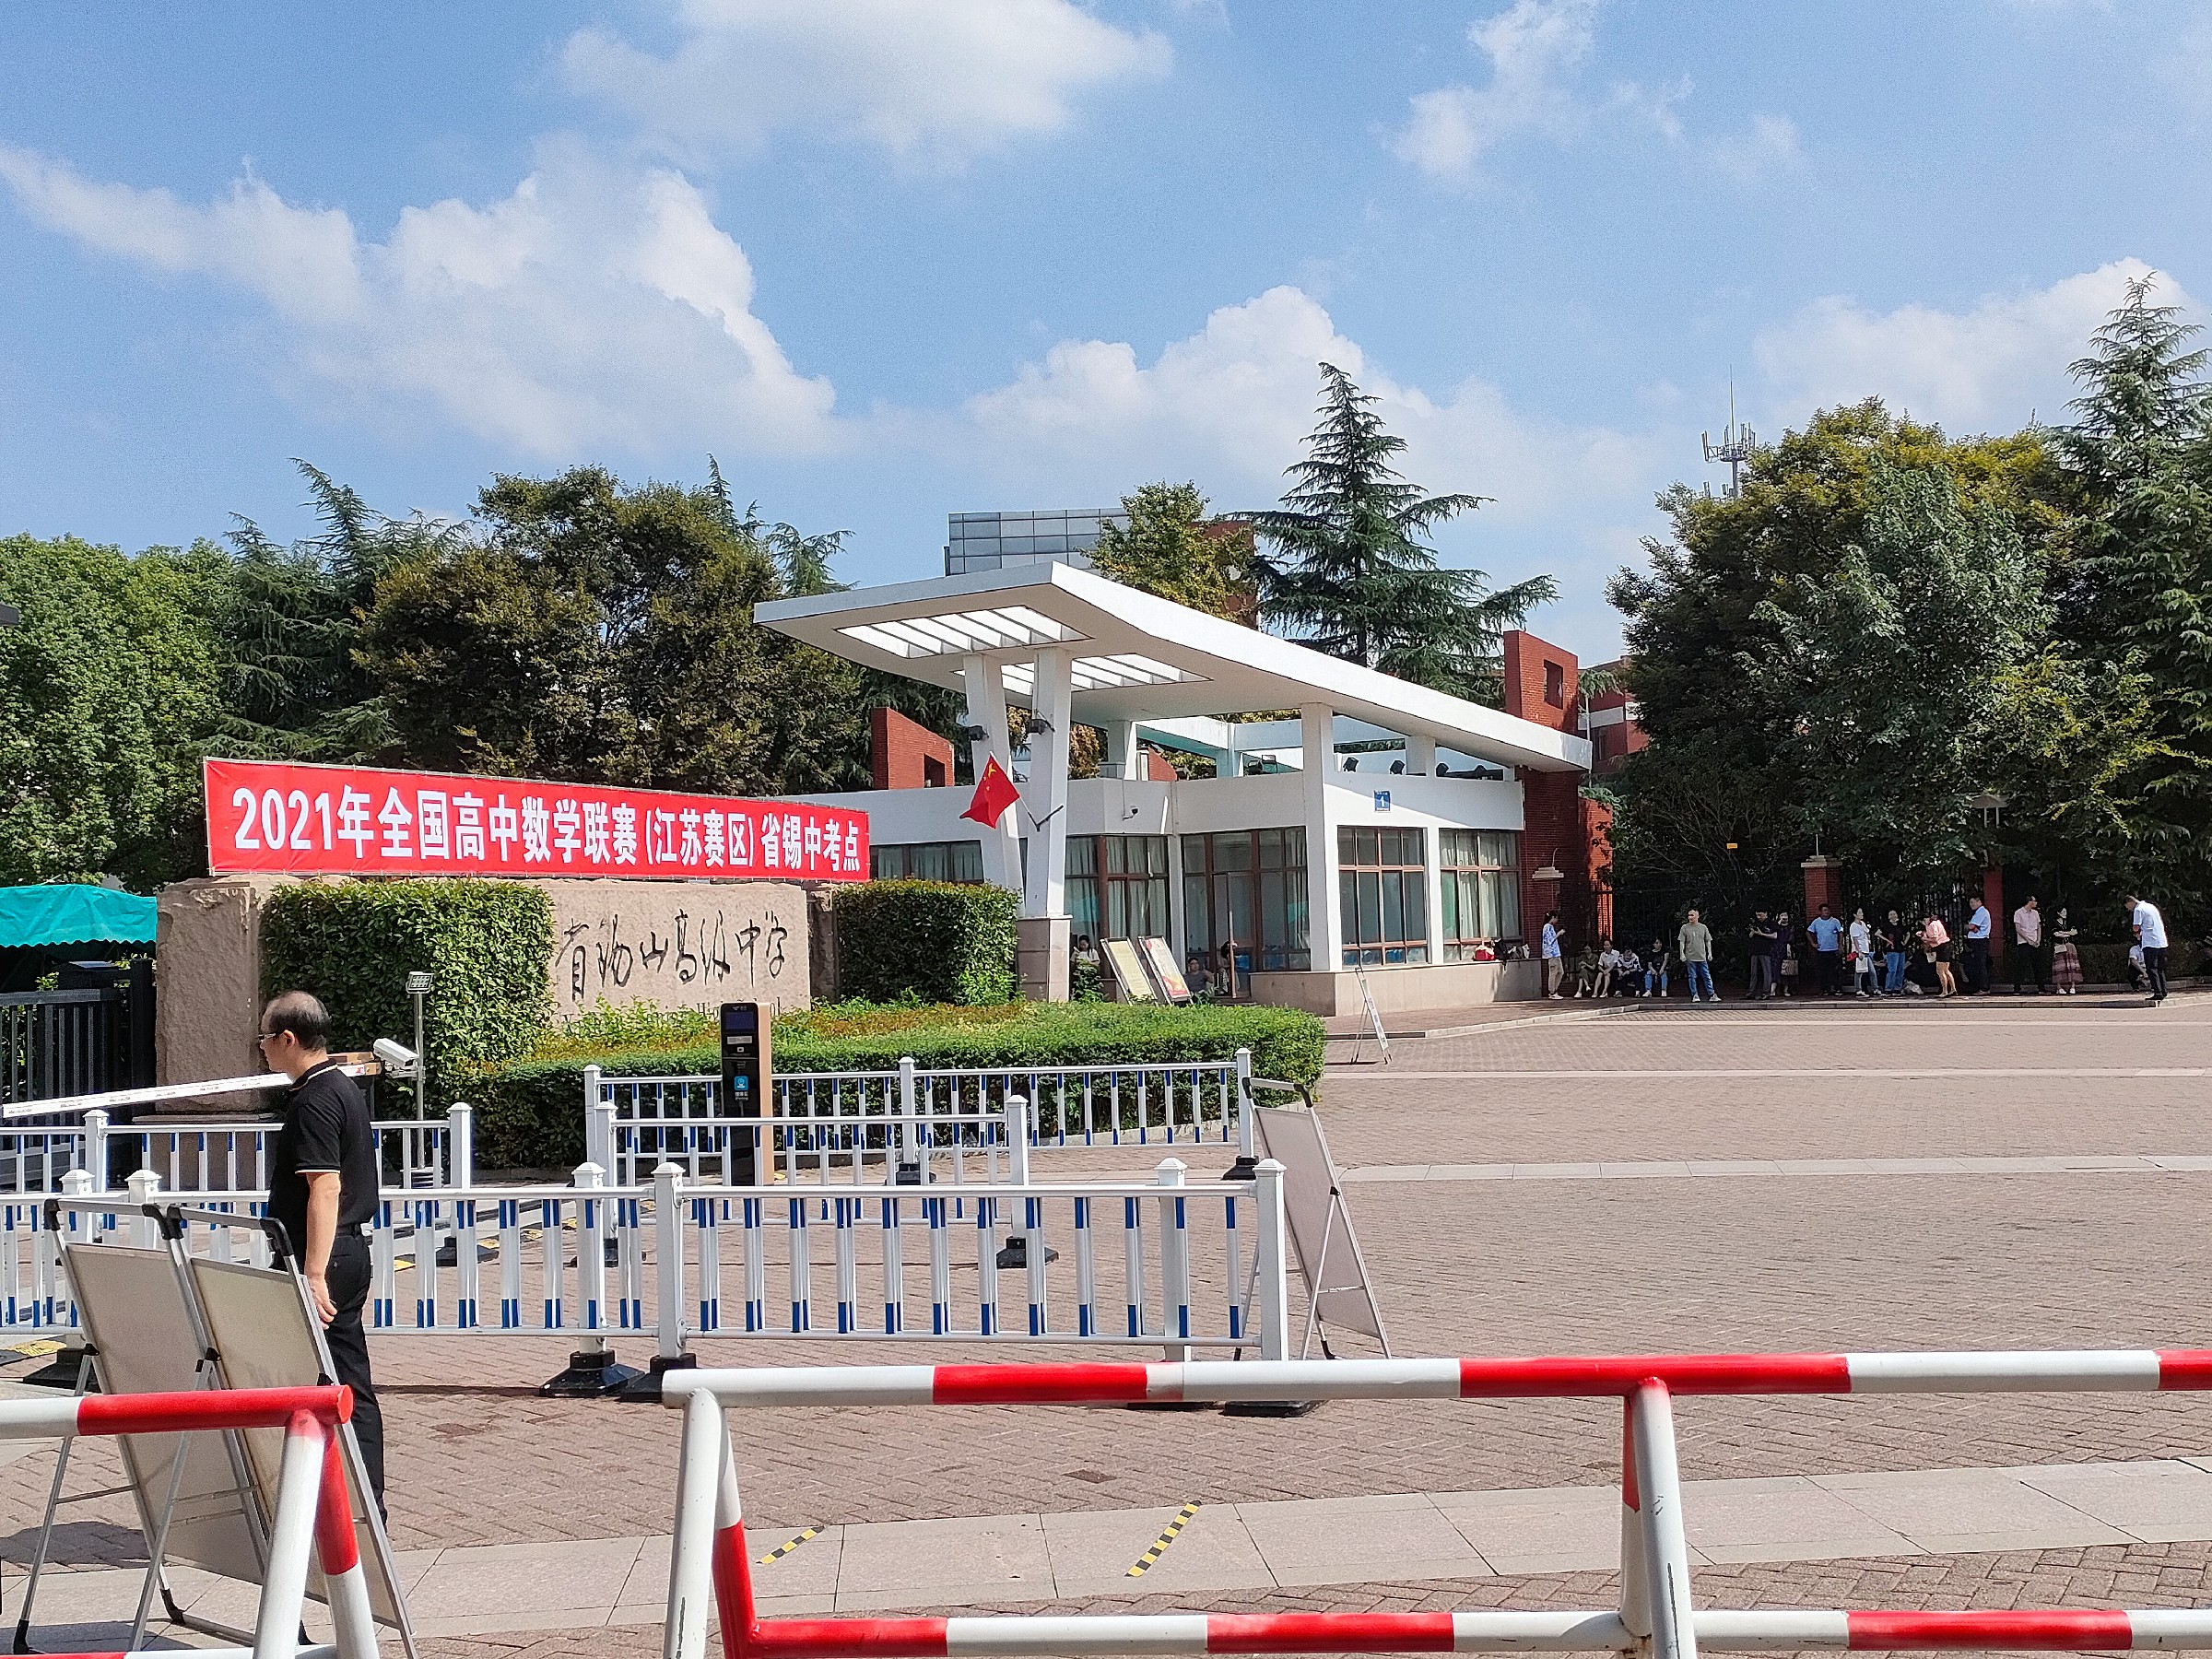
\includegraphics[width=6cm]{../测试图/测试加工}
		\color{gray}\caption{测试加工}
	\end{minipage}
\end{figure}

这三张图的测试结果如表3
\begin{table} [h]
	\centering
	\caption{测试结果}
	\begin{tabular}
		{cccc}
		\toprule[1pt]
		\rowcolor[gray]{0.9} 图片 &测试原图 &测试模糊 &测试加工\\
		\midrule
		准确率   &0.940 &0.695 &0.954\\
		\bottomrule[1pt]
	\end{tabular}
\end{table}

模型对原图的测试是准确的。

很显然,模糊化对测试结果的隐形较大。这里我采用的模糊方式是有损压缩,具体算法可能是取平均值。

另一方面,AI加工的图像给了模型更高的把握。果然只有AI能抗衡AI,我人眼真的看不出有啥大区别。

\subsection{图像裁切}
我考虑训练集具有动物,人物,建筑等的分类,于是我裁切原图,产生了人物(图16),文字(图17),建筑(图18)三块内容:
\begin{figure}[h]
	\centering
	\begin{minipage}[t]{0.3\linewidth}
		\centering
		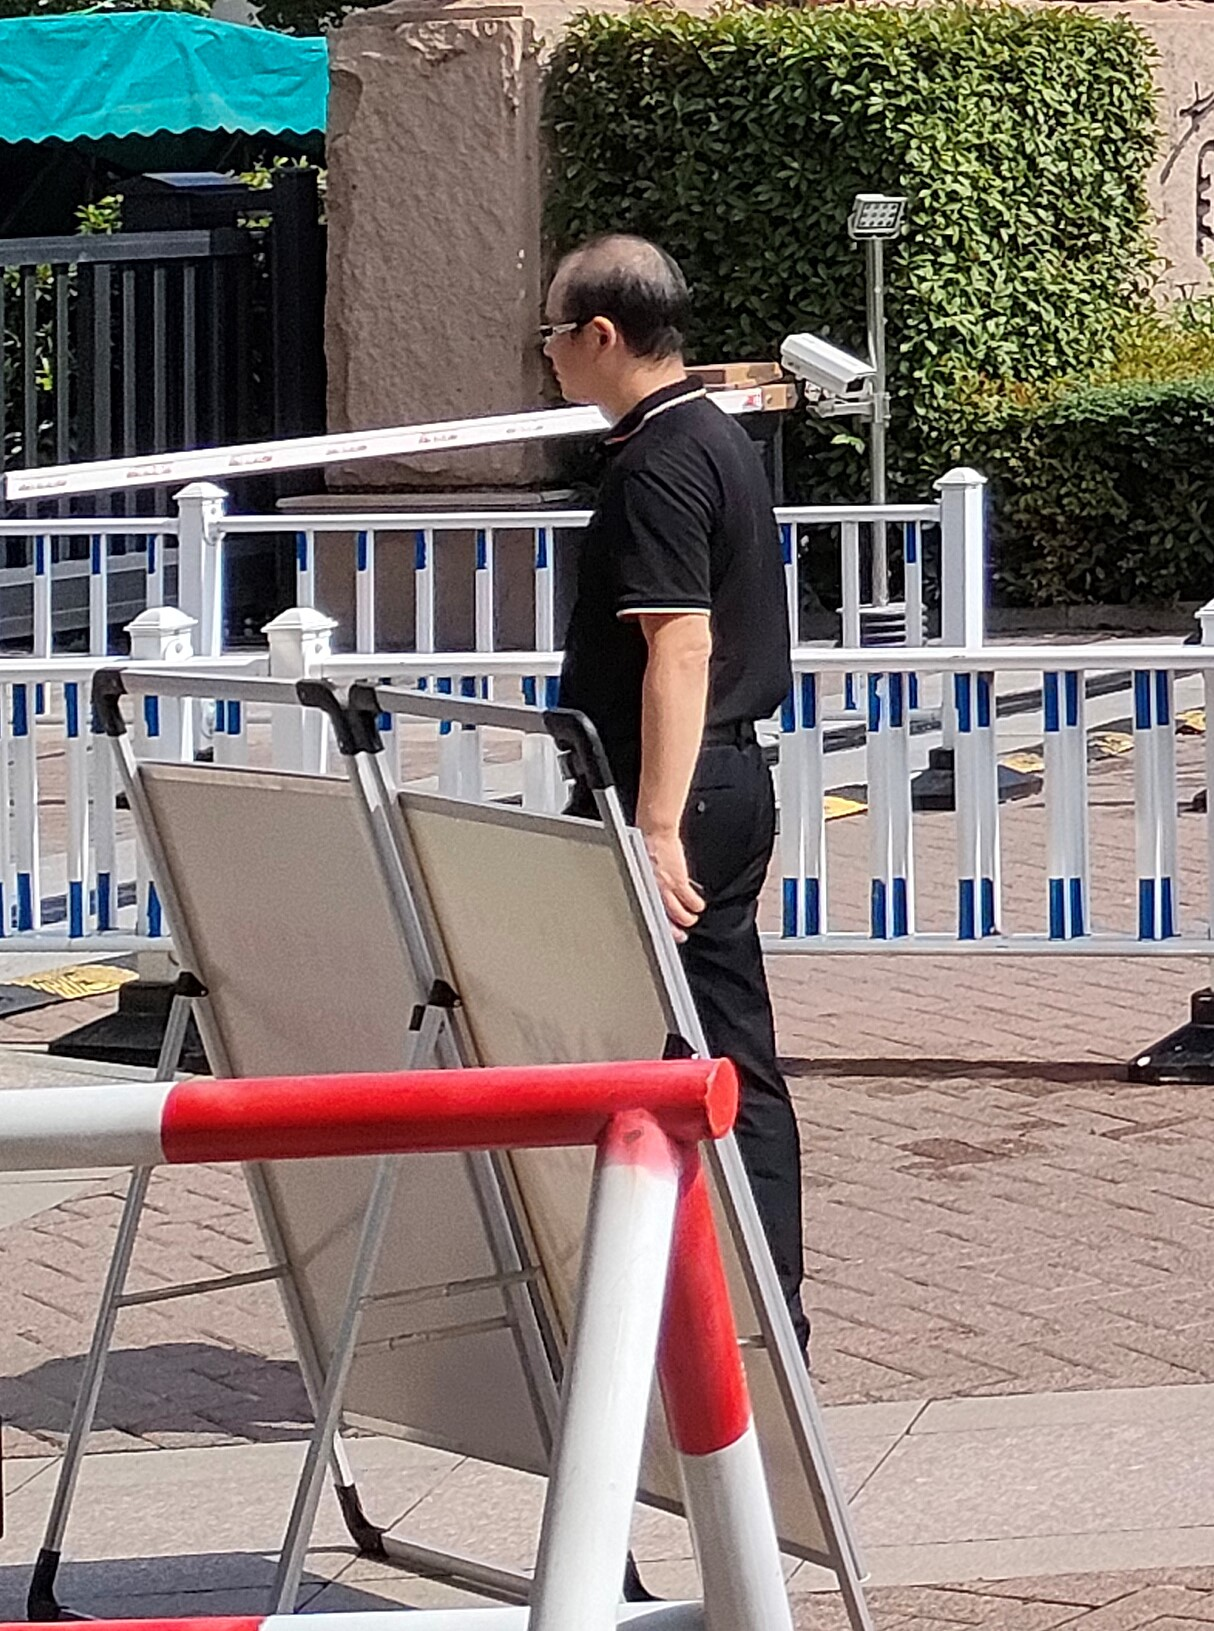
\includegraphics[width=3.5cm]{../测试图/测试裁切1}
		\color{gray}\caption{测试裁切1}
	\end{minipage}
	\begin{minipage}[t]{0.3\linewidth} %图片占用一行宽度的45%
		\centering
		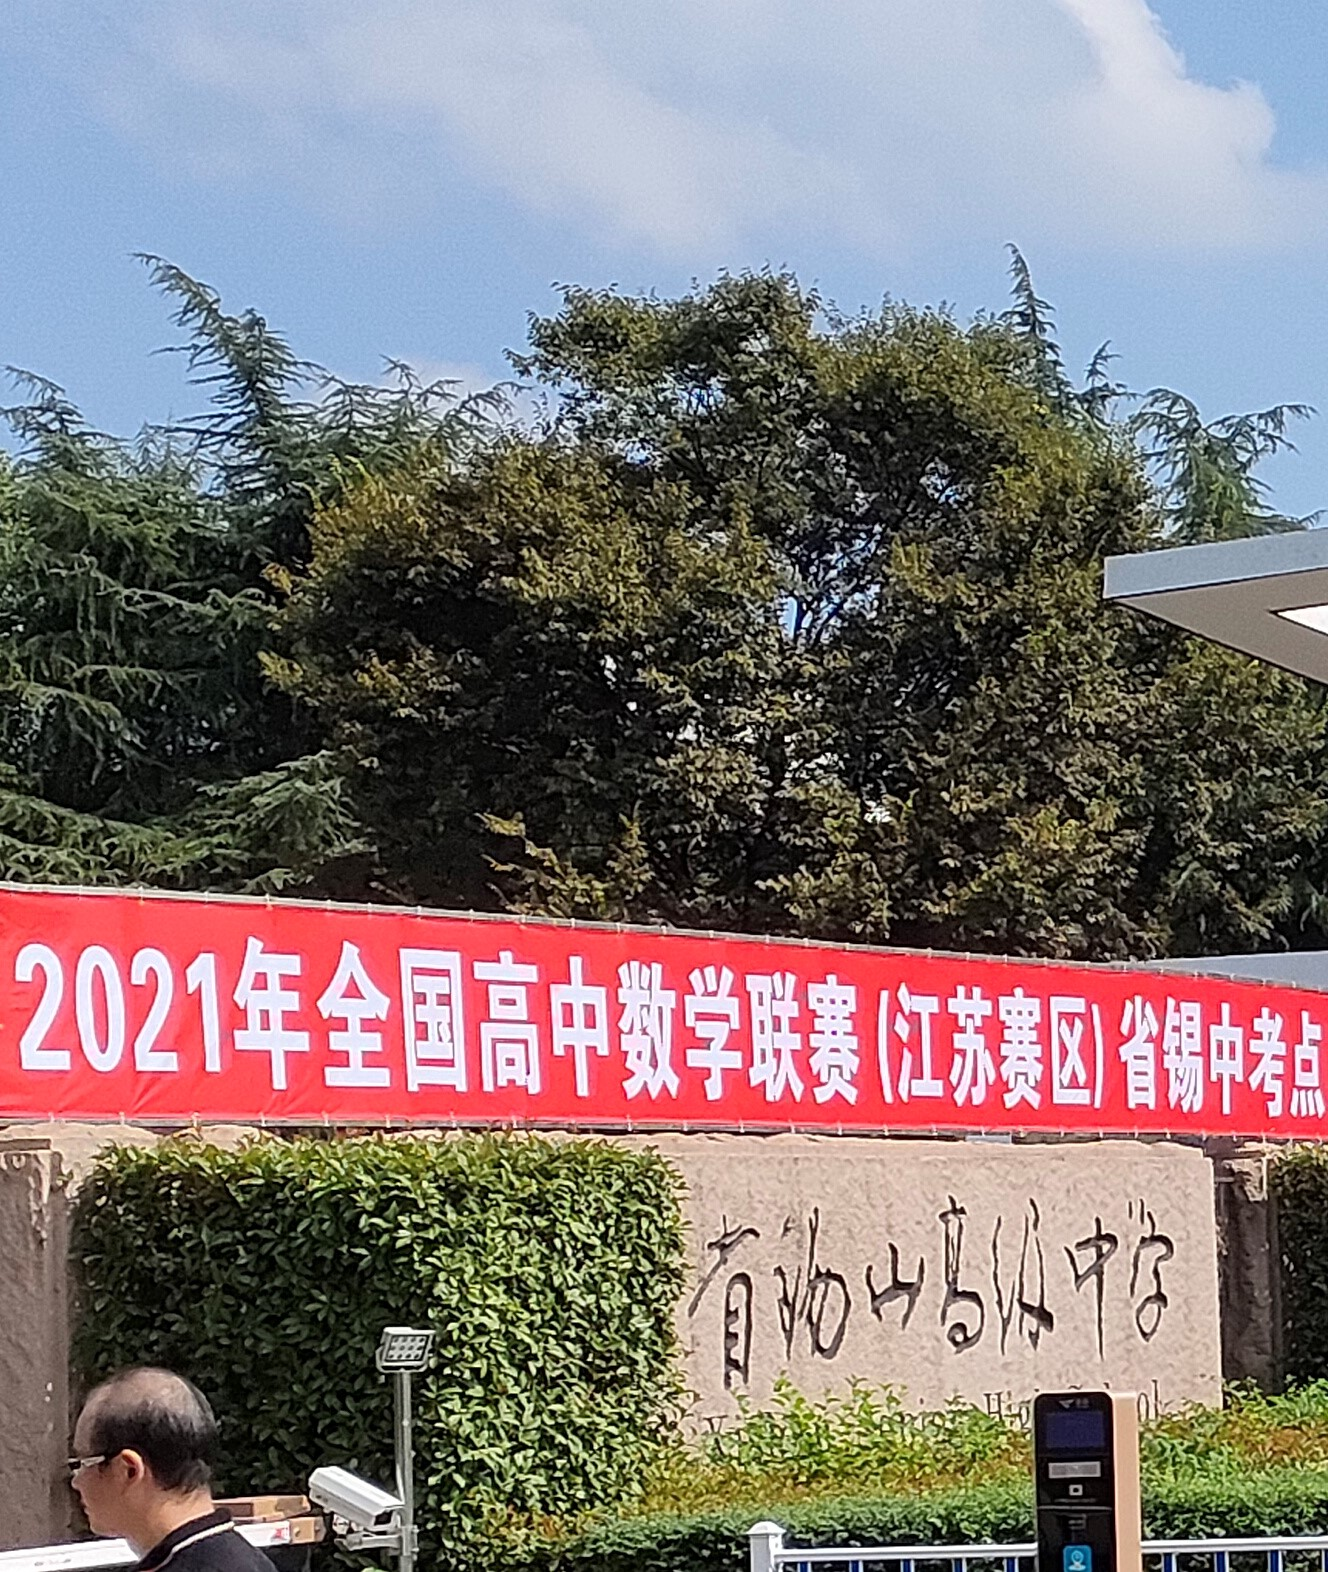
\includegraphics[width=4cm]{../测试图/测试裁切2}
		\color{gray}\caption{测试裁切2}
	\end{minipage}
	\begin{minipage}[t]{0.3\linewidth} %图片占用一行宽度的45%
		\centering
		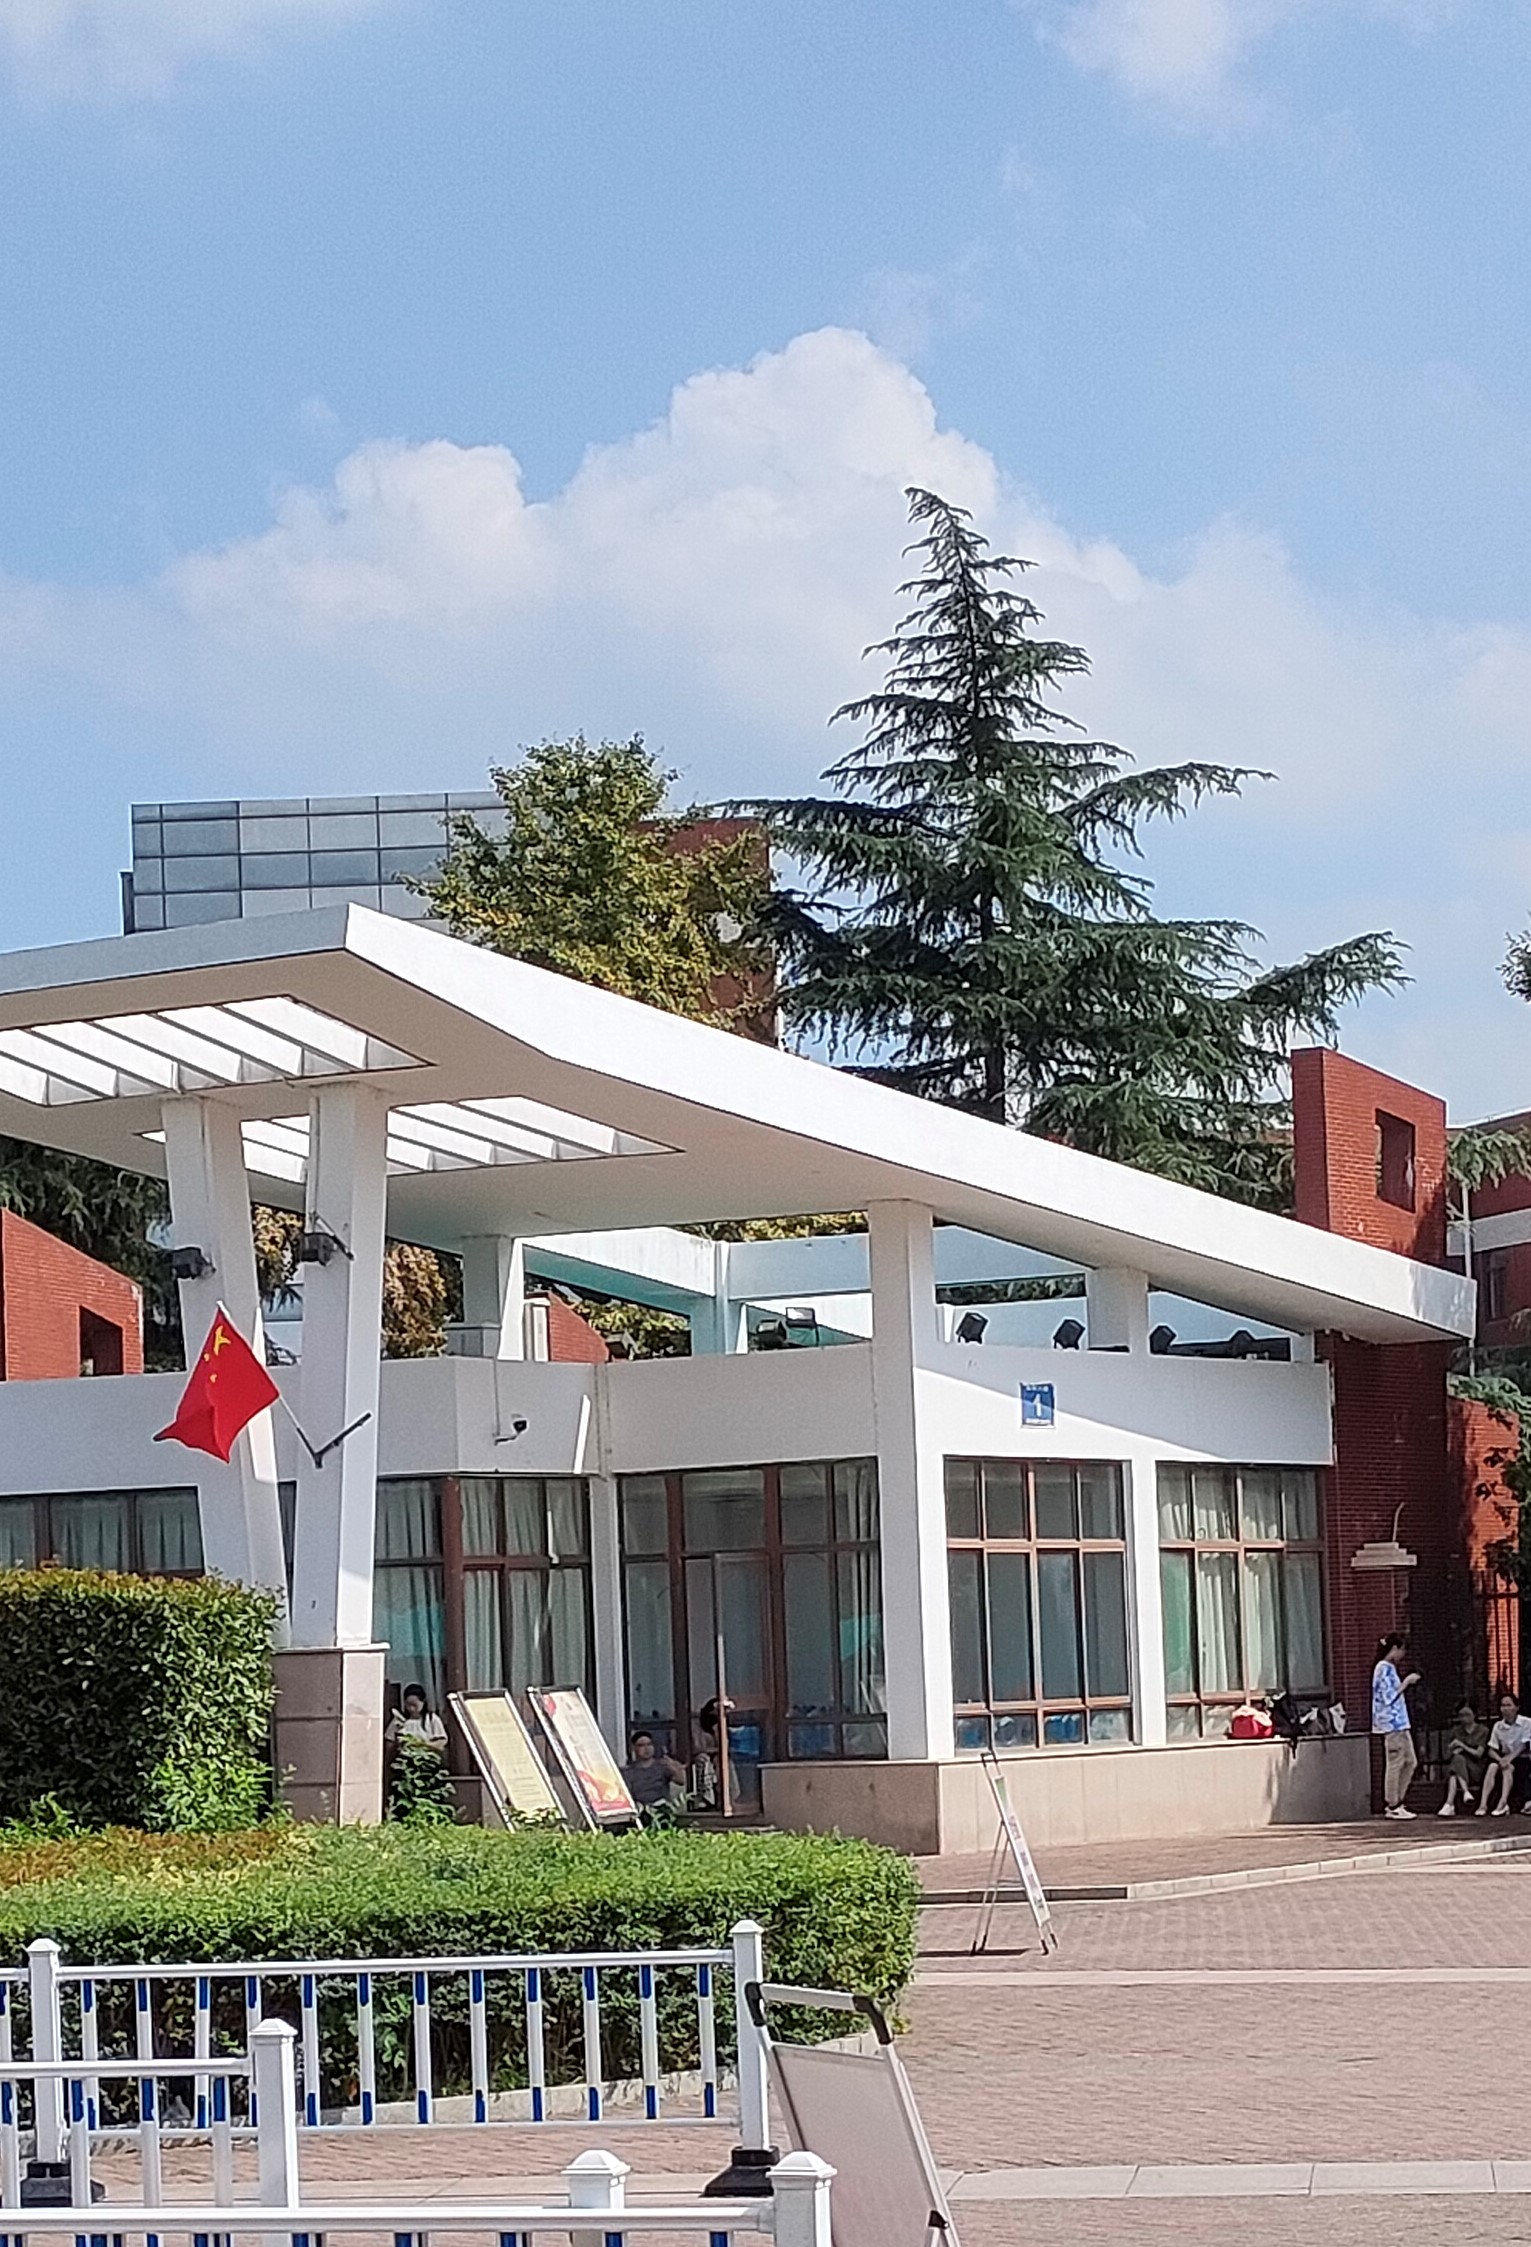
\includegraphics[width=3.5cm]{../测试图/测试裁切3}
		\color{gray}\caption{测试裁切3}
	\end{minipage}
\end{figure}

\begin{table} [h]
	\centering
	\caption{测试结果}
	\begin{tabular}
		{cccc}
		\toprule[1pt]
		\rowcolor[gray]{0.9} 图片 &测试裁切1 &测试裁切2 &测试裁切3\\
		\midrule
		准确率   &0.930 &0.924 &0.247\\
		\bottomrule[1pt]
	\end{tabular}
\end{table}

可以发现,同一张图片内部差异巨大。推测是由于测试裁切3中建筑物轮廓分明,又明显界限,所以被判断是假的。同时,这也间接证明了清晰度的作用。

\subsection{P图}
我尝试了从图19到图23的几种假图。
\begin{figure}[h]
	\centering
	\begin{minipage}[t]{0.3\linewidth}
		\centering
		\includegraphics[width=4cm]{../测试图/测试p1}
		\color{gray}\caption{测试1}
	\end{minipage}
	\begin{minipage}[t]{0.3\linewidth} %图片占用一行宽度的45%
		\centering
		\includegraphics[width=4cm]{../测试图/测试p2}
		\color{gray}\caption{测试2}
	\end{minipage}
	\begin{minipage}[t]{0.3\linewidth} %图片占用一行宽度的45%
		\centering
		\includegraphics[width=4cm]{../测试图/测试p3}
		\color{gray}\caption{测试3}
	\end{minipage}\\
	\begin{minipage}[t]{0.3\linewidth}
		\centering
		\vspace{2mm}
		\includegraphics[width=4cm]{../测试图/测试p4}
		\color{gray}\caption{测试4}
	\end{minipage}
	\begin{minipage}[t]{0.3\linewidth} %图片占用一行宽度的45%
		\centering
		\vspace{2mm}
		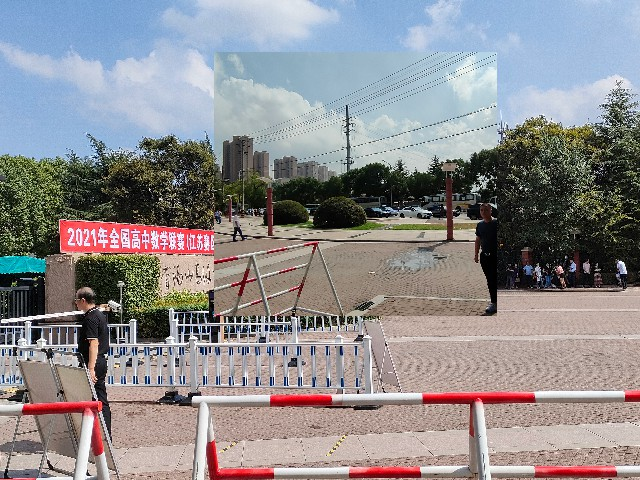
\includegraphics[width=4cm]{../测试图/测试p5}
		\color{gray}\caption{测试5}
	\end{minipage}
\end{figure}

\begin{table} [h]
	\centering
	\caption{测试结果}
	\begin{tabular}
		{cccccc}
		\toprule[1pt]
		\rowcolor[gray]{0.9} 图片 &测试1 &测试2 &测试3 &测试4 &测试5\\
		\midrule
		准确率   &0.926 &0.919 &0.912 &0.985 &0.995\\
		\bottomrule[1pt]
	\end{tabular}
\end{table}

测试1模仿了fake样本P图方式,测试2是人工细致P图,测试3是P图加调光。预测结果均错误。看来清晰度的差别明显影响了模型性能。
测试4为离谱P图,测试5是测试4的模糊版本。模型给出了非常高的把握。

\subsection{小结}
由于训练集清晰度不高,在测试清晰图片时,相当于测试了一个巨大的模糊图片,结果很可能由于图片的大部分real而掩盖了少部分fake,产生误差。
\end{document}
